\documentclass[a4paper,12pt]{article}
\usepackage[utf8]{inputenc}
\usepackage[francais]{babel}
\usepackage[T1]{fontenc}
\usepackage{graphicx}
\usepackage[colorlinks,urlcolor=blue]{hyperref} %hyperlinks
\usepackage{xcolor} %color text
\usepackage[amsthm]{ntheorem} %theorems and co.
\usepackage{amsmath} %mathematical symbols
\usepackage{enumitem} %change numbers into letters in enumerate
\usepackage[normalem]{ulem}

\newenvironment{mld}
  {\par\begin{minipage}{\linewidth}\begin{tabular}{rp{0.7\linewidth}}}
  {\end{tabular}\end{minipage}\par}
\newcommand{\relat}[1]{\textsc{#1}}
\newcommand{\attr}[1]{\emph{#1}}
\newcommand{\prim}[1]{\uline{#1}}
\newcommand{\foreign}[1]{\#\textsl{#1}}
\theoremstyle{remark}
\newtheorem*{remark}{\textbf{Remarque}}

\newcommand{\tabitem}{~~\llap{\textbullet}~~}

\title{HLIN511 -- Projet : \textbf{application de covoiturage}}
\author{Bachar RIMA -- 21511308\\ Ohtmane Farajallah -- 21509759}
\date{\today{}}

\begin{document}
\pagestyle{plain}

\maketitle
{
  \hypersetup{linkcolor=black}
  \tableofcontents
}

\newpage

\section*{Modèle EA}
\label{sec:modele_EA}
\addcontentsline{toc}{section}{\nameref{sec:modele_EA}}

\begin{figure}[!ht]
  \centering
  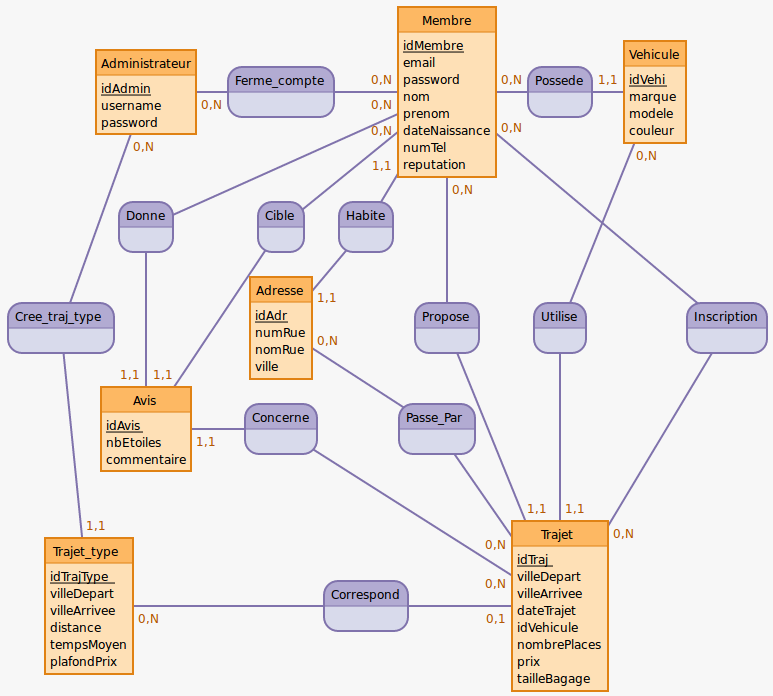
\includegraphics[scale=0.5]{images/modele_EA.png}
  \caption{Modèle Entité-Association}
\end{figure}

\section*{Modèle Relationnel}
\label{sec:modele_relationnel}
\addcontentsline{toc}{section}{\nameref{sec:modele_relationnel}}

\begin{mld}
  \textbf{Administrateur} & (\prim{idAdmin}, \attr{username}, \attr{password})\\
  \textbf{Adresse} & (\prim{idAdr}, \attr{numRue}, \attr{nomRue}, \attr{ville})\\
  \textbf{Membre} & (\prim{idMembre}, \attr{email}, \attr{password}, \attr{nom}, \attr{prenom}, \attr{dateNaissance}, \attr{numTel}, \attr{reputation}, \foreign{idAdr})\\
  \textbf{Vehicule} & (\prim{idVehi}, \attr{marque}, \attr{modele}, \attr{couleur}, \foreign{idProprio})\\
  \textbf{Ferme\_Compte} & (\foreign{\prim{idAdmin}}, \foreign{\prim{idMembre}}, \attr{typeFermeture}, \attr{dureeFermeture})\\
  \textbf{Trajet\_Type} & (\prim{idTrajType}, \attr{villeDepart}, \attr{villeArrivee}, \attr{distance}, \attr{tempsMoyen}, \attr{plafondPrix}, \foreign{idAdmin})\\
  \textbf{Trajet} & (\prim{idTraj}, \attr{villeDepart}, \attr{villeArrivee}, \attr{dateTrajet}, \foreign{idVehiUtilise}, \attr{nbPlaces}, \attr{prix}, \attr{tailleBagages}, \foreign{idConducteur}, \foreign{idTrajType})\\
  \textbf{Inscription} & (\foreign{\prim{idPassager}}, \foreign{\prim{idTraj}})\\
  \textbf{Avis} & (\prim{idAvis}, \attr{nbEtoiles}, \attr{commentaire}, \foreign{idTraj}, \foreign{idDonneur}, \foreign{idCible})\\
  \textbf{Passe\_par} & (\foreign{\prim{idTraj}}, \foreign{\prim{idAdr}})\\
\end{mld}

\section*{Contraintes de Modélisation}
\label{sec:contraintes}
\addcontentsline{toc}{section}{\nameref{sec:contraintes}}

\section*{Triggers et Procédures}
\label{sec:triggers}
\addcontentsline{toc}{section}{\nameref{sec:triggers}}

\end{document}
